
\section{Collider Definitions and Coordinate Systems}

\section{The Large Hadron Collider}

\section{The ATLAS Detector}

\section{Event Reconstruction}
\label{sec:event_reconstruction}

\subsection{Tracks}

\subsection{Jets}

For example, the differentiable cross-section of the ($2\rightarrow n+1$) process in \Cref{fig:quark_gluon} in the extreme soft and collinear limits factorizes into a $2 \rightarrow n$ process times a $1 \rightarrow 2$ split.
In this extreme limit the probability for soft-colinear gluon emission is given by,
\begin{equation}
	\label{eq:gluon_emission}
	d \mathcal{S} = \frac{2 \alpha_s C_F}{\pi} \frac{d \theta}{\sin\theta} \frac{dE}{E} \frac{d\phi}{2\pi},
\end{equation}
where $C_F = \sfrac{4}{3}$ is the color factor for the quarks, $\theta$ is the angle of the emitted gluon with respect to the quark, $E$ is the energy of the emitted gluon, and $\phi$ is the azimuthal angle.

\subsubsection{Particle Flow}
\label{sec:particle_flow}

\section{Event Simulation}

\section{Flavour Tagging}

A diagram of the GN1 model is shown in \Cref{fig:gn1}.

\begin{figure}
    \centering
    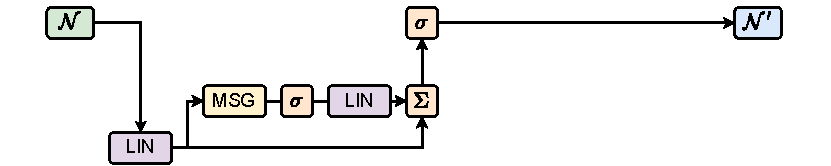
\includegraphics[width=0.99\textwidth]{figures/atlas/gn1.png}
    \caption{Schematic diagram of the GN1 model from Ref.~\cite{GN1}.}
    \label{fig:gn1}
\end{figure}
